%!TEX root = ../dissertation.tex
\clearpage
\begingroup
\setstretch{1}
\iftoggle{DissertateColophonImage}{%
    \begin{center}
    \vspace*{20pt}
    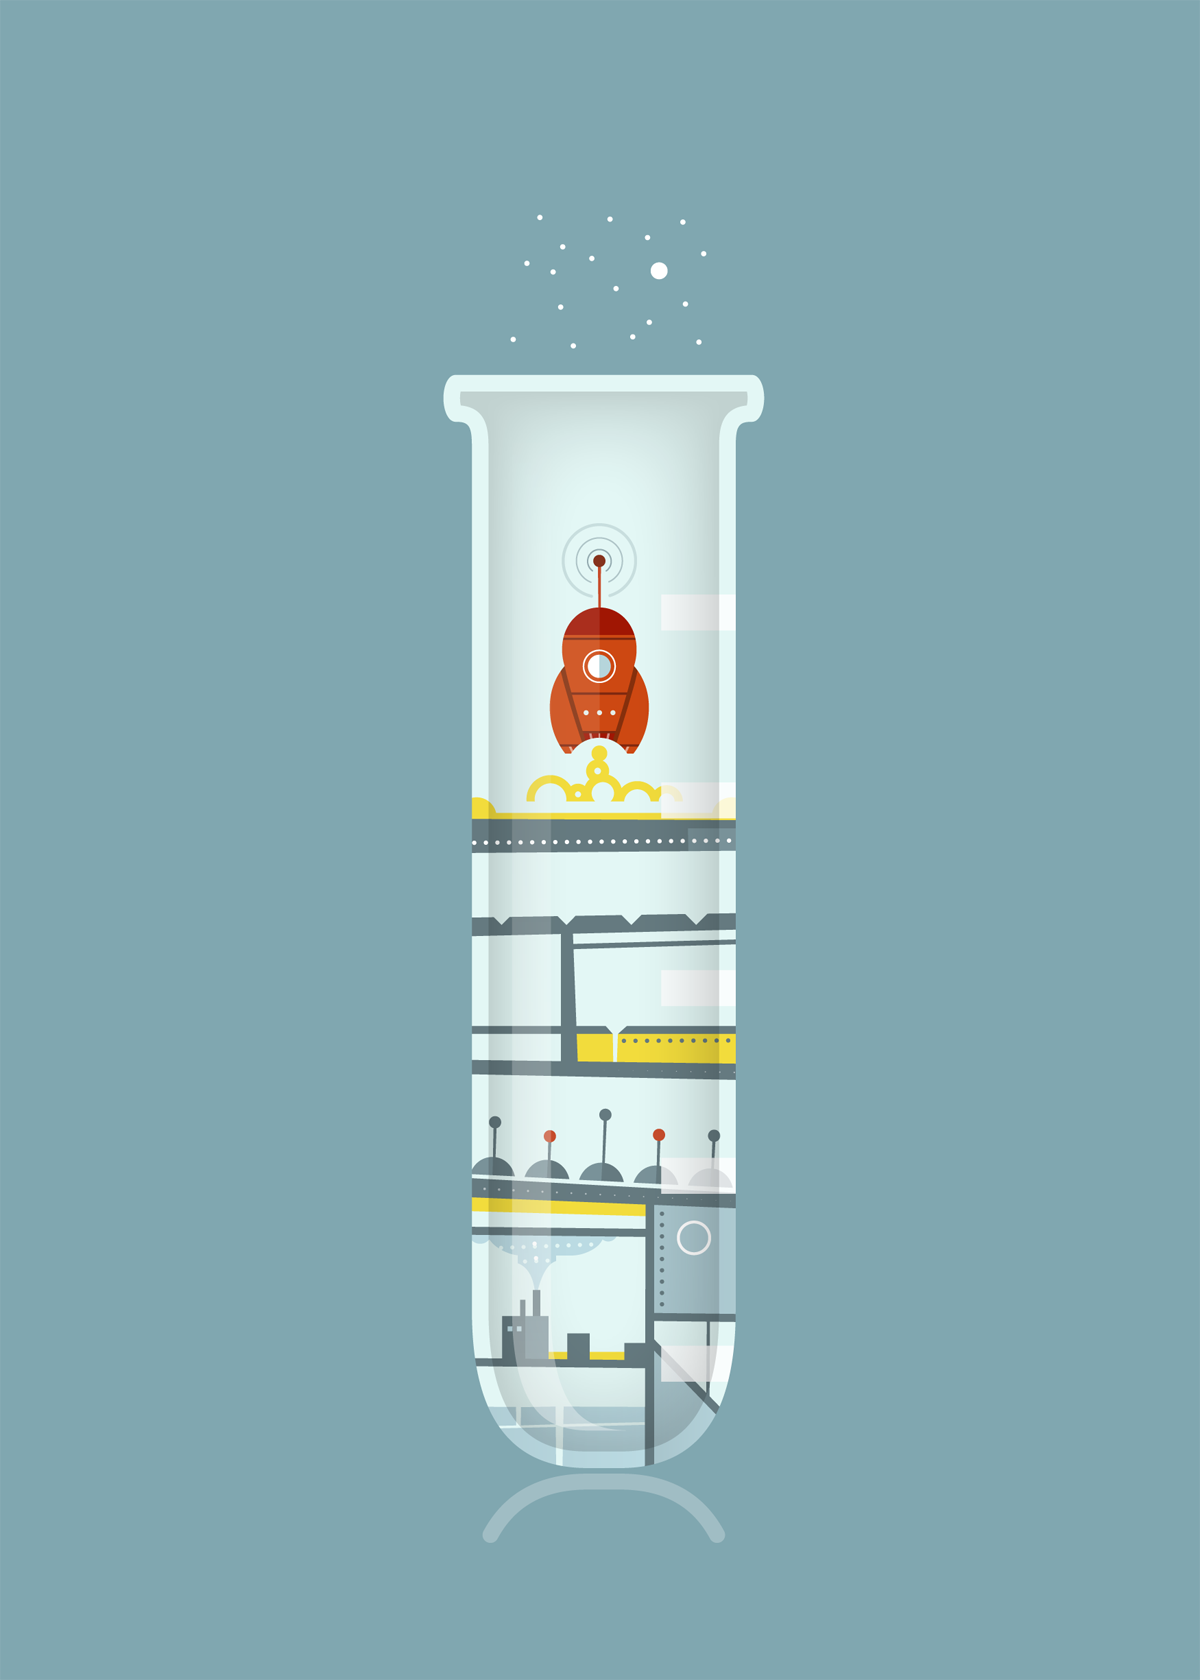
\includegraphics[width=0.42\textwidth]{endmatter/colophon.png}
    \end{center}
}{\vspace*{100pt}}
\begin{center}
\parbox{200pt}{\lettrine[lines=3,slope=-2pt,nindent=-4pt]{\textcolor{SchoolColor}{T}}{his \dissertatedocumentname\ was typeset} with XeLaTeX using Dissertate. The body text is set in \dissertatebodyfont. Dissertate is available at \href{https://github.com/suchow/Dissertate}{github.com/suchow/Dissertate} under the GNU Affero General Public License, version 3.
\iftoggle{DissertateColophonImage}{\par\medskip The illustration, \textit{Science Experiment 02}, was created by Ben Schlitter and released under \href{https://creativecommons.org/licenses/by-nc-nd/3.0/}{CC BY-NC-ND 3.0}.}{}
}
\end{center}
\endgroup
